\documentclass{beamer}
\usetheme{TTU}
\usefonttheme{serif}
\usepackage[T1]{fontenc}
\usepackage[utf8]{inputenc}
\usepackage{mathptmx}
\usepackage{url}
\usepackage{graphicx}
\usepackage{setspace}
\usepackage{esint}
\usepackage[natbibapa]{apacite}
\usepackage{color}
\usepackage{amsmath}
\usepackage{amsfonts}
\usepackage{bm}
\usepackage{Sweavel}
\usepackage{listings}

\def\Sweavesize{\scriptsize}
\def\Rcolor{\color{black}}
%\def\Routcolor{\color{red}}
\def\Rcommentcolor{\color{violet}}
\def\Rbackground{\color[gray]{0.85}}
\def\Routbackground{\color[gray]{0.85}}

\lstset{tabsize=2, breaklines=true, style=Rstyle}



\newcommand{\red}[0]{\textcolor{red}}
%\newcommand{\violet}[0]{\textcolor{violet}}
\newcommand{\green}[0]{\textcolor{green}}
\newcommand{\blue}[0]{\textcolor{blue}}
\newcommand{\comment}[1]{}
\newcommand{\kfold}[0]{\emph{K}-fold cross-validation}

\title[Lecture 3]{Lecture 3: More Missing Data Basics}

\author{Kyle M. Lang}

\institute[TTU IMMAP]{
  Institute for Measurement, Methodology, Analysis \& Policy\\
  Texas Tech University\\
  Lubbock, TX
}

\date{September 8, 2015}


\begin{document}

\setkeys{Gin}{width=\textwidth}
  
\input{sweaveFiles/lecture3-001}


% Use a custom background template for the title slide
{\usebackgroundtemplate{\rule{0pt}{3.4in}\hspace*{2.25in}
    \makebox[0pt][r]{
\includegraphics[natwidth=1000bp, natwidth=283bp,width=2in]{TTU_Logo.png}}}
  
  \begin{frame}[plain]
    
    \titlepage
    
  \end{frame}
}% CLOSE Custom Background Template



\begin{frame}{Outline}
  
  \begin{itemize}
  \item More on missing data mechanisms
    \vspace{12pt}
  \item A few more missing data diagnostics
    \vspace{12pt}
  \item Ad Hoc techniques and their problems
    \vspace{12pt}
  \item More on MI and FIML
  \end{itemize}
  
\end{frame}

\begin{frame}{Missing Data Mechanisms}

  MCAR:
  \begin{align*}
    P(R | Y_{mis}, Y_{obs}) = P(R)
  \end{align*}
  MAR:
  \begin{align*}
    P(R | Y_{mis}, Y_{obs}) = P(R | Y_{obs})
  \end{align*}
  MNAR:
  \begin{align*}
    P(R | Y_{mis}, Y_{obs}) \neq P(R | Y_{obs})
  \end{align*}
  
\end{frame}


\begin{frame}{Simulate Some Toy Data}
  
\begin{Schunk}
\begin{Sinput}
 nObs <- 1000 # Sample Size
 pm <- 0.3 # Proportion Missing
 sigma <- matrix(c(1.0, 0.5, 0.0,
                   0.5, 1.0, 0.3,
                   0.0, 0.3, 1.0),
                 ncol = 3)
 simDat <- as.data.frame(rmvnorm(nObs, c(0, 0, 0), sigma))
 colnames(simDat) <- c("y", "x", "z")
 x <- simDat$x
 y <- simDat$y
 z <- simDat$z
 cor(y, x) # Check correlation between X and Y
\end{Sinput}
\begin{Soutput}
[1] 0.4691526
\end{Soutput}
\end{Schunk}


\end{frame}


\begin{frame}[allowframebreaks]{MCAR Example}
  
\begin{Schunk}
\begin{Sinput}
 ## Simulate MCAR Missingness:
 rVec1 <- as.logical(rbinom(nObs, size = 1, prob = pm))
 mean(rVec1) # Check the PM
\end{Sinput}
\begin{Soutput}
[1] 0.301
\end{Soutput}
\begin{Sinput}
 y2 <- y
 y2[rVec1] <- NA
 cor(y2, x, use = "pairwise") # Look at correlation
\end{Sinput}
\begin{Soutput}
[1] 0.4744126
\end{Soutput}
\begin{Sinput}
 
\end{Sinput}
\end{Schunk}


\input{sweaveFiles/lecture3-004}
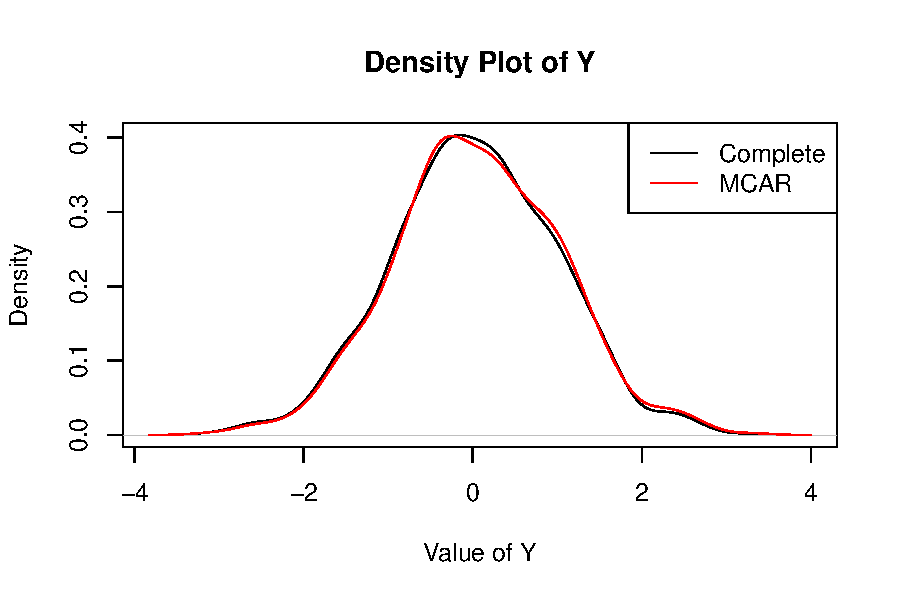
\includegraphics{sweaveFiles/lecture3-004}

\end{frame}


\begin{frame}[allowframebreaks]{MAR Example}
  
\begin{Schunk}
\begin{Sinput}
 ## Simulate MAR Missingness:
 rVec2 <- pnorm(x, mean = mean(x), sd = sd(x)) < pm
 mean(rVec2)
\end{Sinput}
\begin{Soutput}
[1] 0.287
\end{Soutput}
\begin{Sinput}
 y3 <- y
 y3[rVec2] <- NA
 cor(y3, x, use = "pairwise") # Not looking so good :(
\end{Sinput}
\begin{Soutput}
[1] 0.3715953
\end{Soutput}
\begin{Sinput}
 ## MI to the rescue:
 miceOut1 <- mice(data.frame(y3, x),
                  m = 100,
                  maxit = 1,
                  method = c("norm", ""),
                  printFlag = FALSE)
 impList1 <- list()
 for(m in 1 : miceOut1$m) {
     impList1[[m]] <- complete(miceOut1, m)
 }
 corList <-lapply(impList1,
                  FUN = function(impDat){
                      cor(impDat$x, impDat$y3)
                  }
                  )
 mean(unlist(corList)) # Oh, much nicer :)
\end{Sinput}
\begin{Soutput}
[1] 0.4835711
\end{Soutput}
\end{Schunk}


\input{sweaveFiles/lecture3-006}
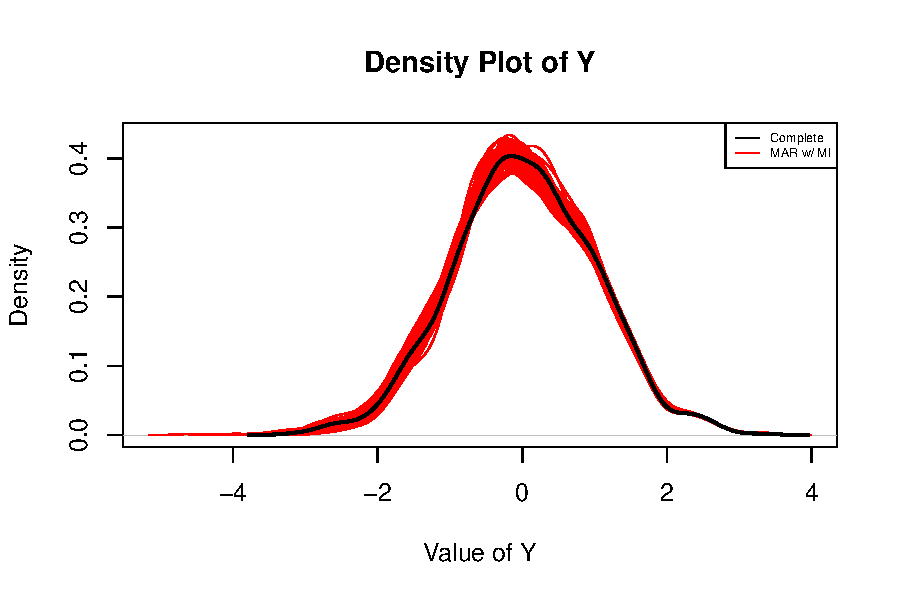
\includegraphics{sweaveFiles/lecture3-006}

\end{frame}


\begin{frame}[allowframebreaks]{MNAR Example}
  
\begin{Schunk}
\begin{Sinput}
 ## Simulate MNAR Missingness:
 rVec3 <- pnorm(y, mean = mean(y), sd = sd(y)) < pm
 mean(rVec3)
\end{Sinput}
\begin{Soutput}
[1] 0.294
\end{Soutput}
\begin{Sinput}
 y4 <- y
 y4[rVec3] <- NA
 cor(y4, x, use = "pairwise") # Hmm...looks pretty bad.
\end{Sinput}
\begin{Soutput}
[1] 0.3708081
\end{Soutput}
\begin{Sinput}
 ## Can MI help?
 miceOut2 <- mice(data.frame(y4, x),
                  m = 100,
                  maxit = 1,
                  method = c("norm", ""),
                  printFlag = FALSE)
 impList2 <- list()
 for(m in 1 : miceOut2$m) {
     impList2[[m]] <- complete(miceOut2, m)
 }
 corList2 <-lapply(impList2,
                  FUN = function(impDat){
                      cor(impDat$x, impDat$y4)
                  }
                  )
 mean(unlist(corList2)) # Not really
\end{Sinput}
\begin{Soutput}
[1] 0.3914519
\end{Soutput}
\begin{Sinput}
 
\end{Sinput}
\end{Schunk}


\input{sweaveFiles/lecture3-008}
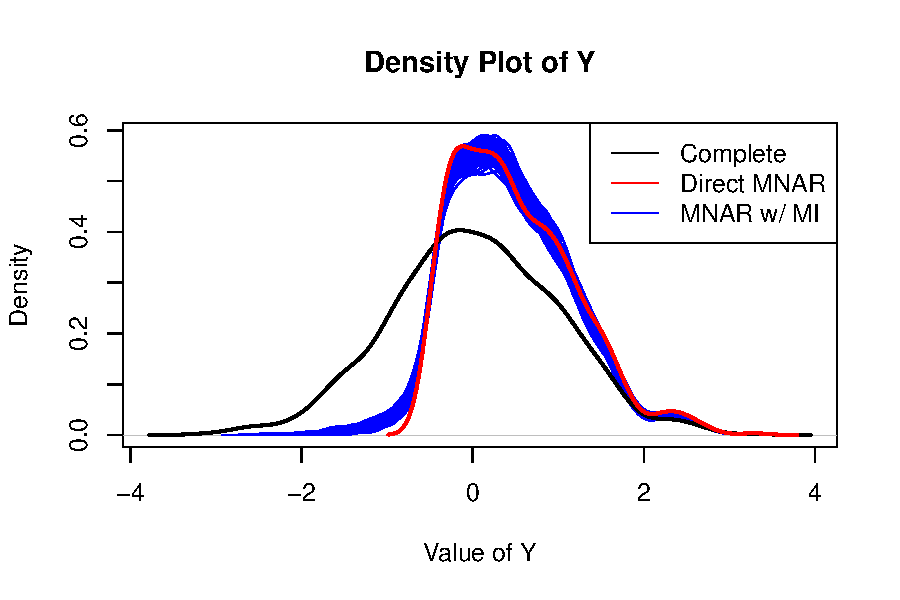
\includegraphics{sweaveFiles/lecture3-008}

\end{frame}


\begin{frame}[allowframebreaks]{Indirect MNAR Example}
  
  \textsc{Question:} In our previous MAR example, what happens if we don't account for the predictor of the MAR missingness?
    
\begin{Schunk}
\begin{Sinput}
 cor(y3, x, use = "pairwise") # Hmm...that's a problem.
\end{Sinput}
\begin{Soutput}
[1] 0.3715953
\end{Soutput}
\end{Schunk}


\textsc{Answer:} We get \emph{Indirect MNAR.}

\input{sweaveFiles/lecture3-010}
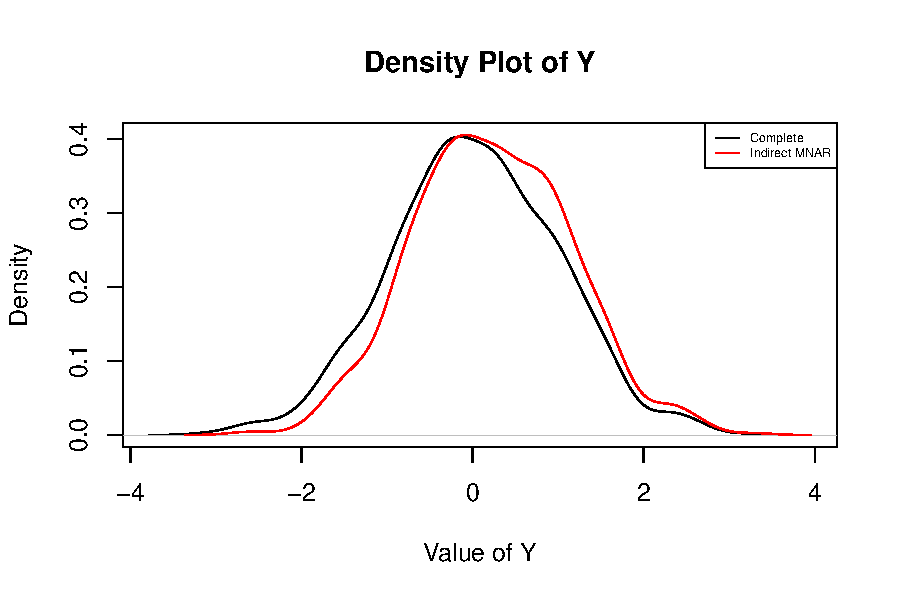
\includegraphics{sweaveFiles/lecture3-010}

\end{frame}


\begin{frame}[allowframebreaks]{Tricky Example}
  
  \textsc{Question:} What happens if we ignore the predictor of missingness, but that predictor is independent of our study variables?
    
\begin{Schunk}
\begin{Sinput}
 rVec3 <- pnorm(z, mean = mean(z), sd = sd(z)) < pm
 y5 <- y
 y5[rVec3] <- NA
 cor(y5, x, use = "pairwise")
\end{Sinput}
\begin{Soutput}
[1] 0.472859
\end{Soutput}
\end{Schunk}


\textsc{Answer:} We get back to MCAR :)

\input{sweaveFiles/lecture3-012}
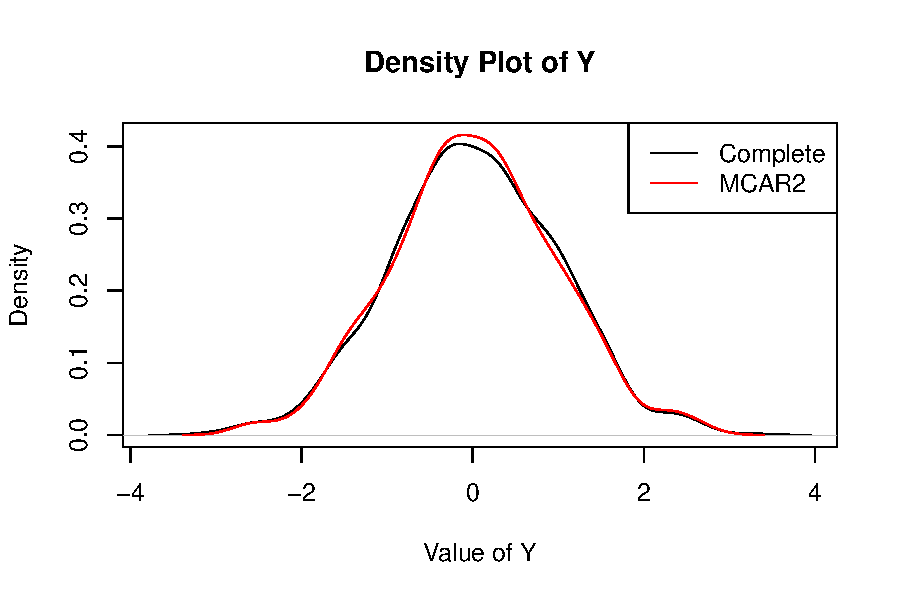
\includegraphics{sweaveFiles/lecture3-012}
  
\end{frame}

\end{document}
